\documentclass[10pt]{article}
\usepackage{titlesec}
\usepackage{titling}
\usepackage[margin=0.8in]{geometry}
\usepackage{graphicx}
\usepackage{hyperref}
\usepackage[export]{adjustbox}


\titleformat{\section}
{\large }
{}
{0.0em}
{\bfseries \uppercase}

\titleformat{\subsubsection}[runin]
{\large \bfseries \uppercase}
{}
{0em}
{}

\titlespacing{\subsubsection}
{0em}{0em}{0em}

\renewcommand{\maketitle}{
	\begin{center}
	{\bfseries \Huge
	\theauthor}
	\rule{17.5cm}{1pt}
	\end{center}	
}

\begin{document}

	% Name
	\author{Prakash Sanyasi}
	\maketitle
	
	% Address,Contact information (Contact,e-mail), Photograph 
	\begin{minipage}{0.5\linewidth}
		\href{http://cst.edu.bt/}{\bf College of Science and Technology} \\
		{\bf Rinchending : Phuntsholing} \\
		{\bf Chhukha : Bhutan}\\ \\
		{\bf Contact: } (+975) 17965898 \\
		{\bf Email: } \href{mailto:prakashsanyasi619@gmail.com}{\tt prakashsanyasi619@gmail.com} \\
	\end{minipage}
	\begin{minipage}{0.45\linewidth}
		\raggedleft
		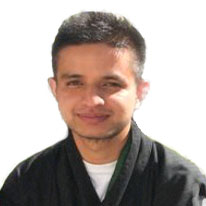
\includegraphics[width=0.4\textwidth]{cover_photo}
	\end{minipage}

	\vspace{0.5cm}
	%Career Objective
	\section{Objectives}
	\begin{itemize}
		\item  To learn and contribute to the world’s technical innovations and to improve the lifestyle of mankind through technology.
		\item  To study systems used in IIT Bombay and want to implement such systems in our country.
	\end{itemize}
	
	%Education
	\section{Education}
	\begin{center}  
		\begin{tabular}{ | l | l | l | l |}
			\hline
			\textbf{Examination} & \textbf{College/School}  & \textbf{Passing Year} & \textbf{Pass Percentage}\\ \hline
			BE in IT &College of Science and Technology &---\- & ---\-\\ \hline
			12\textsuperscript{th} Grade BCSEA & Mongar Higher Seondary School & 2014 & 72\% \\ \hline
			10\textsuperscript{th} Grade BCSEA & Mongar Higher Seondary School & 2012 & 78\% \\ \hline
		\end{tabular}
	\end{center}

	%Project
	\section{Projects}
	\begin{enumerate}
		\item {\bf Home Automation Using IoT}\\
		I am currently working on this project. This is first hardware based project done by IT students as final year project. We are using arudio mega-2560, esp8266 wifi module and other sensors to automated the ight and other home appliances. We had own created a local server, back-end and moblie application to controls this system.
		\item {\bf Find Law App}\\
		We had built a mobile application which acts as a repository of the laws of our country such as acts, conventions, constitutions, rules and court judgements. It also consists backend whereby admin can add, edit and updates the content of the mobile application. Admin can also notify the user when their in changes in laws.
	
	\end{enumerate}
 
	%Training Intership
	\section{TRAINING \& INTERNSHIP}
	\begin{itemize}
		\item  I did 45 days of Of Job Training at Bhutan Power Cooperations Litmited where I learned about networking and also did particle like optical fiber maintenance.
		\item I had worked as a developer for more than one month in office of the attorney general whereby we developed find law app.
	\end{itemize}

	%Research publications
	\section{RESEARCH PUBLICATIONS}
	\begin{enumerate}
		\item We did a research on "Awareness of Cyber Crime in Bhutan" and had published the paper in International Conference on Emerging Technologies of Information and Communication, ETIC 2019.
	\end{enumerate}
\end{document}